\documentclass[../main.tex]{subfiles}

\begin{document}

\section{Overview}

Any system which aims to generate queries to fulfill an aim or process will be necessarily limited in utility if it operates with only a single static database schema. Within the health domain, data structures and vocabularies are increasingly complex and diverse, and systems capable of generalizing to other data models and institutions stand to be more impactful. Even the OMOP common data model, though widely used, is often updated to include custom database tables and data to fulfill various project-specific needs \cite{belenkaya2021extending, peng2021towards, zoch2021adaption, warner2019hemonc, zhou2013evaluation, shin2019genomic, kwon2019development}. 

This chapter explores what we call a Semantic Metadata Mapping, or SMM, which we leverage as a data-model agnostic means of generating queries for eligibility criteria. Section 6.2 explores related work. Section 6.3 discusses SMM structure and configuration. Section 6.4 summarizes the work of this chapter.

\section{Related Work}

Many recent efforts at creating machine-readable data and resources for cross-system communication originate with the Semantic Web \cite{berners2001semantic}, a set of standards undergirded by ontologies, taxonomies, and inference rules designed for the Internet. As explained by the creators of the Semantic Web:

\begin{quote}
\textit{"An ontology may express the rule "If a city code is associated with a state code, and an address uses that city code, then that address has the associated state code." A [Semantic Web] program could then readily deduce, for instance, that a Cornell University address, being in Ithaca, must be in New York State, which is in the U.S., and therefore should be formatted to U.S. standards."} \cite{berners2001semantic}
\end{quote}

The logic behind data model-agnostic query generation using an SMM is similar. For example, suppose an eligibility criteria specifies that patients identify as Hispanic. If an SMM contains a database column, $IsHispanic$, where a given tuple of value "1" means the tuple represents the UMLS concept of Hispanic (C0086409), a program can deduce then that a SQL query with a WHERE clause of \textit{"WHERE IsHispanic = 1"} should retrieve patients who identify as Hispanic. This relatively simple logic is inspired by concepts of the Semantic Web and forms the basis of SMMs. Where SMMs differ most clearly, however, is the use of the UMLS as a means of managing metadata. To the best of our knowledge, this is the first project to do so to enable database query generation.

Using metadata for the purpose of generating database queries has been explored in previous research. Bizer and Seaborne \cite{bizertreating} demonstrated that a simple ontology of database schema elements could be used to automatically generate SQL queries. Sequeda \textit{et al} proposed similar methods using First Order Logic and and created a publicly available rule engine for the research community \cite{sequeda2009direct,sequeda2011survey}. Knoblock \textit{et al} and Gupta \textit{et al} demonstrated the potential of such method for integrating heterogeneously structured databases of protein, gene, and metabolic pathway data \cite{knoblock2012semi, gupta2015karma}.

\section{Methods}

An SMM includes a listing of available databases, tables, columns, and so on within a given database schema. These database artifacts are "tagged" using a subset of UMLS concepts, many from the National Cancer Institute (NCI) and Health Level 7 (HL7) vocabularies. Examples of categories and concepts possible within an SMM include:

\begin{itemize}
    \item \textbf{Demographic} - Age (C0001779), Ethnic Group (C00015031), Language (C0023008), Female (C0086287), Male (C0086582), Transgender (C3266856), Hispanic (C0086409). 
    \item \textbf{Identifiers} - Patient (C5236161), Encounter (C3865224)
    \item \textbf{Metadata} - Concept Mapping (C3858752), Code (C0805701), Code System (C2347818), Quantitative Value (C0392762).
    \item \textbf{Polarity} - Normal (C0205307), Abnormal (C0205161), Positive (C1514241), Negative (C0205160), Low (C0205251), High (C0205250).
    \item \textbf{Vital Status} - Living (C4551704), Deceased (C0011065).
\end{itemize}

Alternatively, a column may also be tagged using a UMLS Source Abbreviation, or SAB, such as ICD-10, SNOMED, LOINC, or RXNORM. Tagging a column as an SAB indicates that the tuple contents of a column represent codes associated with a given source system. For example, a column which contains diagnosis codes such as E11.62, I25.10, and others (ICD-10 codes) would have an SAB tag of "ICD10CM". SABs supported by our SMMs are:

\begin{itemize}
    \item \textbf{Current Procedural Terminology (CPT)}
    \item \textbf{Healthcare Common Procedure Coding System (HCPCS)}
    \item \textbf{ICD-9}
    \item \textbf{ICD-10}
    \item \textbf{ICD-10 Procedure Coding System (ICD-10 PCS)}
    \item \textbf{LOINC}
    \item \textbf{National Drug File (NDC)}
    \item \textbf{NCI}
    \item \textbf{RxNorm}
    \item \textbf{SNOMED}
\end{itemize}

A column tagged by a UMLS concept or SAB can also be conditional, or in other words, only true given some other logic also being true. For example, Table \ref{tbl_smm_example_data} shows a hypothetical database table of diagnosis codes. Column $code$ contains codes from various vocabularies, including ICD-9, ICD-10, and SNOMED.

\def\arraystretch{0.8}
\begin{table}[h!]
\centering
\begin{tabular}{l l l l}
 \toprule
 \textbf{patient\_id} & \textbf{coding\_system} & \textbf{code} & \textbf{dx\_name} \\
 \hline
    1 & ICD-10 & I50 & Heart Failure \\
    2 & ICD-10 & E87.70 & Fluid Overload \\
    3 & SNOMED & 4270721002 & AIDS Associated Disorder \\
    4 & ICD-9  & 493.0 & Asthma \\
 \hline
\end{tabular}
\caption{Hypothetical database table for patient diagnoses. Codes from a variety of different vocabularies are shown under the $coding\_system$ column.}
\label{tbl_smm_example_data}
\end{table}

In this case, $code$ would be tagged with 3 conditional SABs, ICD-9, ICD-10, and SNOMED, with each SAB tag's condition defined as a SQL WHERE clause in the form of a string. For example, the "ICD10CM" tag would be paired with the condition, "WHERE coding\_system = 'ICD-10'". This is a machine-readable equivalent of, "The $code$ column represents an ICD-10 code only if the $coding\_system$ column in the same record is of value 'ICD-10'". Table \ref{tbl_smm_column_config} shows a more complete configuration example of all 3 SABs for the column.

\def\arraystretch{0.8}
\begin{table}[h!]
\centering
\begin{tabular}{l l l}
 \toprule
 \textbf{ColumnName} & \textbf{SAB} & \textbf{SqlWhere} \\
 \hline
    code & ICD9CM  & coding\_system = 'ICD-9' \\
    code & ICD10CM & coding\_system = 'ICD-10' \\
    code & SNOMED  & coding\_system = 'SNOMED' \\
 \hline
\end{tabular}
\caption{Example SMM configuration for the $code$ column. } 
\label{tbl_smm_column_config}
\end{table}

\begin{figure}[H]
  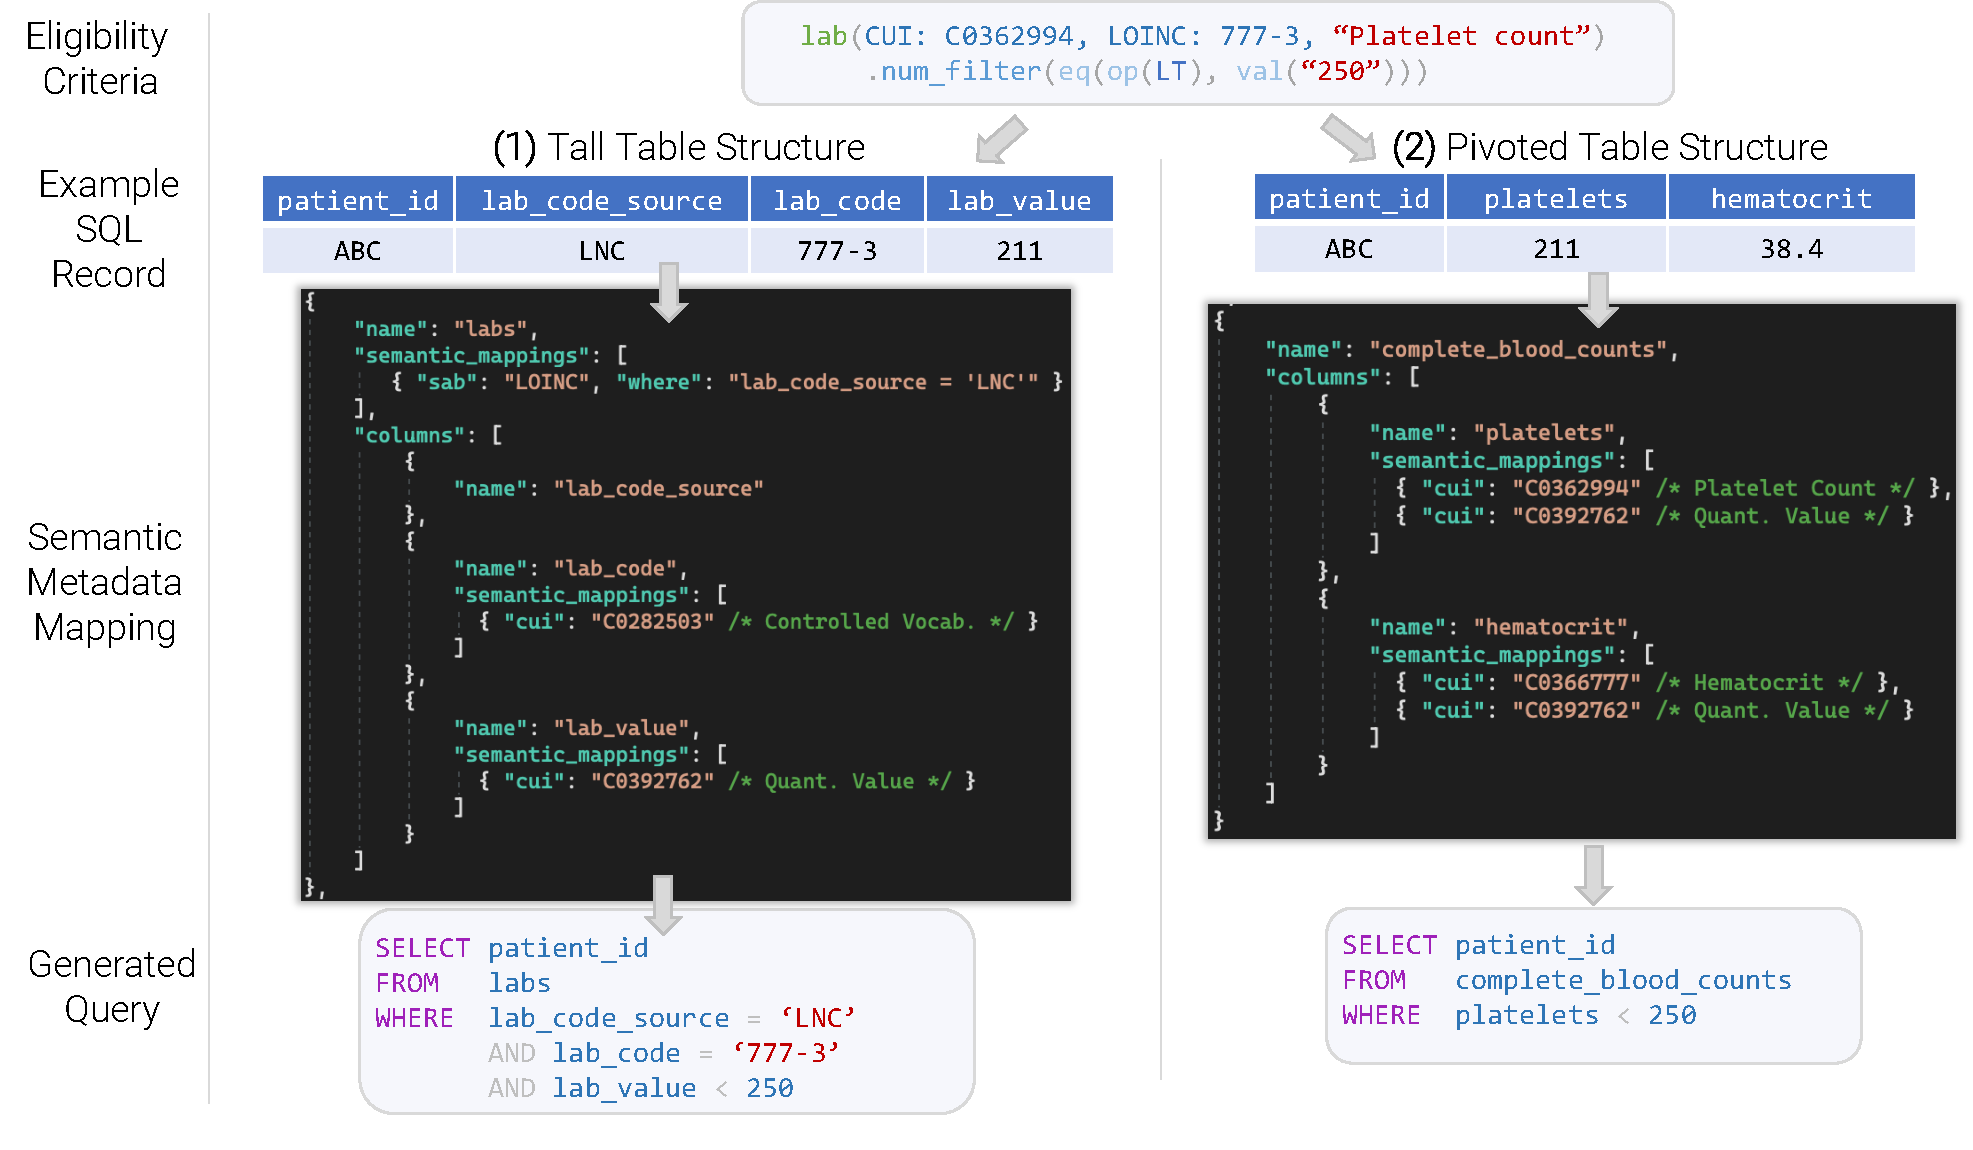
\includegraphics[scale=0.47]{Figures/6_smm/leafai_smm.pdf}  
\caption{Two hypothetical database schema to generate queries for platelet counts (shown in logical form after normalization). This example illustrates the flexibility of our SMM system (represented here in JSON format) in adapting to virtually any data model. On the left, "Tall Table Structure", platelet counts must be filtered from within a general purpose "labs" table. Our KB recognizes that labs may be stored as LOINC codes and the corresponding SMM indicates that records in this table can be filtered to LOINC values. On the right, "Pivoted Table Structure", platelet counts are stored as a specific column in a "complete\_blood\_counts" table, and thus can be directly queried without further filtering. Additional metadata, columns, tables, types and so on needed in SMMs are omitted for brevity.}
\label{fig_leafai_smm}
\end{figure}

The use of UMLS concepts, SABs, and optional conditions for each enables query generation across a wide variety of potential data models and database schema. An example of this can be seen in Figure \ref{fig_leafai_smm}, which shows strategies by which a given criterion can be used to generate schema-specific queries by leveraging different SMMs. In cases where there is more than one means of querying a given concept (e.g., two SQL tables for diagnosis codes), the SMM returns both tables, which may be combined in a UNION statement downstream. The query generation algorithm using an SMM is shown in Algorithm \ref{alg_smm}. SQL queries for the "Tall Table Structure" (left example) in Figure \ref{fig_leafai_smm} would be generated using the $directSqlSets$ array in Algorithm \ref{alg_smm}, while the "Pivoted Table Structure" (right example) would be generated using $encodedSqlSets$. As the algorithm checks for mappings in both cases at runtime, the algorithm does not need to be recompiled to handle different database structures.

\SetKwComment{Comment}{/* }{ */}

\begin{algorithm}
%\KwData{$LogicalForm$}
%\KwData{$SMM$}
\DontPrintSemicolon
%\BlankLine
$directSqlSets \gets []$ \Comment*[l]{SQL from DB columns mapped to specific CUIs}
$encodedSqlSets \gets []$ \Comment*[l]{SQL from DB columns which encode SABs}
\BlankLine
\For{$concept$ in $LogicalForm.concepts$}{
    \BlankLine
    \If{$concept$ in $SMM.columns$}{
        $column \gets SMM.columns[concept]$\;
        $sql \gets GenerateConceptSql(concept, column)$\;
        $directSqlSets.push(sql)$\;
    }
    \BlankLine
    \For{$sab$ in $SMM.sabs$}{
          \If{$concept$ encodable as $sab$}{
            $column \gets SMM.sabs[concept]$\;
            $sql \gets GenerateEncodedSabSql(concept, column)$\;
            $encodedSqlSets.push(sql)$\;
          }
        }
}
$\textbf{return}$ $directSqlSets \cup encodedSqlSets$\;
\caption{Algorithm for generating SQL queries by mapping concepts for a given logical form and SMM. Actual SQL syntax generation steps and certain steps are omitted for brevity. Each concept within a logical form is evaluated for direct mappings to SMM columns within a database and encodable mappings to SABs. $SMM.columns$ and $SMM.sabs$ are dictionaries of UMLS concepts which return zero or one database columns.}\label{alg_smm}
\end{algorithm}

\section{Limitations}

Our SMM implementation is limited in a number of ways, most notably in that our tagging schema is not entirely machine readable. Specifically, the use of optional conditions in the form of SQL WHERE clauses implemented as simple strings (e.g., "WHERE IsPrimaryDx = 1") means that an SMM does not carry granular semantic information of actual filtering logic or tuple-level values, but rather simply trusts that a given SQL condition will filter as expected. A more robust future SMM implementation may annotate tuple-level values semantically at a more granular level, though this would necessarily entail far more work on the part of the annotator in exhaustively describing every possible value of every relevant column in a database.

\section{Summary}

This chapter examined our system for data model-agnostic query generation using SMMs, an encoding system where metadata on various clinical database schema elements are tagged using UMLS concepts and SABs. 

\end{document}